\documentclass{article}

%opening
\title{Simulation of the interaction of a supernova explosion with the ISM}
\author{Cristina Caprioglio}
\date{2023/2024 }
\usepackage[margin=0.75in]{geometry}
	\usepackage{amssymb}
	\usepackage{amsmath}
	\usepackage{multicol}
	\usepackage{graphicx}
	\usepackage{physics}
	\usepackage{subcaption}
	\usepackage{float}
	\usepackage[justification=centering]{caption}
	\usepackage{xcolor}
	\usepackage{calligra}
\usepackage[T1]{fontenc}
\begin{document}

\maketitle

\section*{Introduction}\label{intro}
Supernova explosions are the main responsibles of the stellar feedback in the ISM. They produce a rapid ejection of large quantities of gas in the ISM. The process last a few seconds, with the velocity of the ejected mass being of the order of $10^{3}$\textemdash$10^{4}$ km/s, and it provides the ISM with an energy of $E\sim 10^{51}$ erg. Due to the high velocities of the ejecta, which are supersonic, it causes the quick (a few hundred years) formation of a shock, which expansion generates a roughly spherical shell of shocked ISM: this shell and its interior are called a supernova remnant (SNR). 
The shock propagation is described by the so-called Sedov solution, with the shock radius increasing with time as $R_{shock}\propto t^{2/5}$. Understanding this process is of vital importance in the evolution of the ISM in galaxies, but it's also relevant for AGN feedback process. 
For a more detailed discussion on supernovae, please refer to Cimatti et al.\cite[Sec. 8.7]{cimatti}.\\
In this project, we numerically study the time evolution of a SNR with a simplified model that doesn't take into account radiative losses (so our ISM is uniform,  we have no stellar winds before the explosion, we have no thermal conduction, etc.) by using a hydrocode for the 1D numerical integration of Euler equations. We developed it using Fortran90, while we used gnuplot for the plots.
\section{1D Hydrocode}
The code we use is based on the ZEUS code by J. Stone and M. Norman (see \cite{stone} for more details), and it's an hydrocode for the 1D numerical integration of Euler equations.
\subsection{Description}\label{descrip}
As mentioned above, our code solves the Euler equations of fluid dynamics in 1D. Using Cartesian coordinates, our set is written as:
\begin{align}
	&\pdv{\rho}{t}+\pdv{(\rho v)}{x}=0 \label{eoc}\\
	&\pdv{m}{t}+\pdv{(mv)}{x}+\pdv{p}{x}=0\quad\text{or}\quad\pdv{v}{t}+v\pdv{v}{x}+\frac{1}{\rho}\pdv{p}{x}=0 \label{eom}\\
	&\pdv{\epsilon}{t}+\pdv{(\epsilon v)}{x}+p\pdv{v}{x}=0,\label{eoe}
\end{align}
where $\rho,\, p,\, v,$ and $\epsilon$ are respectively the density, the pressure, the velocity, and the internal energy of the fluid, while $m=\rho v$ is the momentum density. We couple our system with the gas equation of state, which is:
\begin{equation}\label{eqstate}
	\epsilon=\frac{p}{\gamma -1},
\end{equation}
with $\gamma=5/3$ being the adiabatic coefficient for a monoatomic gas.\\
To solve our equations we use a staggered grid, which means that not all quantities are centered at the same points. In our case, we have $m$ and $v$ centered at integer numbers $j$, while $\rho,\,p,$ and $\epsilon$ are centered at half-integer numbers $j+1/2$, so we basically have both $x_{j}$ and $x_{j+1/2}=x_{j}+\frac{1}{2}\Delta x$, where $\Delta x$ is the spatial step. 
Calling a the first grid and b the second one, we define:
\begin{equation*}
	dx_a(j)=x_{j+1}-x_{j} \qquad \text{and} \qquad dx_b(j)=x_{j+1/2}-x_{j-1/2}.
\end{equation*}
We can also use either Cartesian or spherical coordinates, which give us for the volume elements $\Delta x$ and $\Delta r^3/3$ respectively.\\
Since we are dealing with shocks, we need to add a dissipation term, namely an \textit{artificial viscosity} $q$, which mimics the real physical viscosity, given by:
\begin{equation}
	q=
	\begin{cases}
		Q^2 \rho(\Delta x)^2 \abs{\pdv{v}{x}}^2\quad &\text{if} \; \pdv{v}{x}<0,\\
		0 \quad &\text{otherwise},
	\end{cases}
\end{equation} 
with $Q=const$. The artificial viscosity is added to the pressure in the hydro equations, see Von Neumann et al.\cite{vonneuman} for further information.\\
After setting the initial conditions, we can start the time integration, where at the beginning of each cycle we have to compute the timestep $\Delta t$. The latter has to satisfy the Courant-Friedrichs-Lewy (CFL) condition for stability, so we set $\Delta t$ as:
\begin{equation}\label{timeeq}
	\Delta t=C\min_{j}{\frac{x_{j+1/2}-x_{j-1/2}}{\abs{v}+c_{s,j}}} \qquad C\in \left]0,1\right[,
\end{equation}
where $c_s=\sqrt{\gamma p/\rho}$ is the sound speed for an ideal gas. It's worth noting that in theory the addition of artificial viscosity adds another constraint, but we can neglect it. \\
During each cycle we execute two steps: the source one and the transport one. We denote with $j$ the spatial index and with $n$ the temporal one.
\subsubsection{The source step}
During this step we want to update the $v$ and $\epsilon$ arrays using a forward time-centered space (FTCS) scheme. In order to do this, we need three different substep. First, we update the velocity array for the pressure gradient:
\begin{equation}
	v_{j}^{n+1}=v_{j}^n-2\Delta t\left(\frac{p_{j+1/2}^n-p_{j-1/2}^n}{dx_{b,j}(\rho_{j+1/2}^n+\rho_{j-1/2}^n)}\right),
\end{equation}
then we find $q_{j+1/2}$ with:
\begin{equation}
	q_{j+1/2}=
	\begin{cases}
		Q^{2}\rho_{j+1/2}(v_{j+1}-v_j)^2 \quad &\text{if} \; v_{j+1}-v_j<0\\
		0 \quad &\text{otherwise},
	\end{cases}
\end{equation}
and we use it to update both the velocity and the energy:
\begin{align}
	&v_j^{n+1}=v_j^n-\Delta t\left(\frac{q_{j+1/2}^n-q_{j-1/2}^n}{dx_{b,j}(\rho_{j+1/2}^n+\rho_{j-1/2}^n)}\right)\\
	&\epsilon_{+1/2}^{n+1}=\epsilon_{j+1/2}^n-\Delta t\left(\frac{v_{j+1}^n-v_{j-1}^n}{dx_{a,j}}\right).
\end{align}
Lastly, we add the contribution of the compressional heating to $\epsilon$:
\begin{equation}
	\epsilon^{+1}_{j+1/2}=\epsilon^n_{j+1/2}\left[\frac{1-(\Delta t/2)(\gamma -1)(\div{v})_i^n}{1+(\Delta t/2)(\gamma -1)(\div{v})_i^n}\right],
\end{equation}
where $\div{v}$ is defined following Stone \& Norman code (see \cite{stone}).
\subsubsection{The transport step}
The transport terms (which correspond to the second terms in Eq.\eqref{eoc}-\eqref{eoe}) are included using the I order Upwind method. First, we define the momentum density $m$, then we update the density. Once this is done, we proceed to calculate the mass fluxes $f_j$ at the cell interface $x_j$, taking into consideration the sign of $v_j$:
\begin{equation}
	f_j=
	\begin{cases}
		\rho_{j-1/2}v_j \quad &\text{if} \; v_j>0\\
		\rho_{j+1/2}v_j \quad &\text{otherwise}.
	\end{cases}
\end{equation}
We need to do this because the other variables are updated using the so-called \textit{consistent advection} (see \cite[Sec. 4.4]{stone}), which improves the local conservation. \\
\paragraph{}
	The last part of the code concerns the boundary conditions, which depend on the chosen system of coordinates and the used grid. For the variables centered on half-integers we have the same conditions for both Cartesian and spherical coordinates: denoting the variable as $y$, we have that $y_1=y_2$ and $y_{j_{max}}=y_{j_{max}-1}$. These boundary conditions are for traditional outflows, and we apply them at quantities centered on integers in Cartesian coordinates as well. For quantities using grid A in spherical coordinates we need the following BCs: $y_2=0$, $y_1=-y_3$ (reflection), and $y_{j_{max}}=y_{j_{max}-1}$.



\subsection{Tests}
We choose $Q=3.0$ and $C=0.5$. We then proceed to carry on different tests:
\begin{itemize}
	\item Sod shock tube test in Cartesian coordinates with $0\le x \le 1$, $\gamma=1.4$ and $t_{max}=0.245$. Our initial conditions are $\rho=1.0$, $p=1.0$, and $v=0$ if $x\le 0.5$, otherwise we have $\rho=0.125$, $p=0.1$, and $v=0$. The results are plotted in Fig. \ref{fig:cartshock100} and \ref{fig:cartshock1000}, respectively for a grid with 100 and 1000 points.
	\item spherical shock tube in spherical coordinates with $0\le r \le 2$, $\gamma=1.4$ and $t_{max}=0.5$. Our initial conditions are $\rho=1.0$, $p=1.0$, and $v=0$ if $r\le 1$, otherwise we have $\rho=0.125$, $p=0.1$, and $v=0$. The results are plotted in Fig. \ref{fig:spheshock100} and \ref{fig:spheshock1000}, respectively for a grid with 100 and 1000 points.
	\item strong shock tube in Cartesian coordinates with $0\le x \le 1$, $\gamma=5/3$ and $t_{max}=2$. Our initial conditions are $\rho=100$, $p=0.67$, and $v=0$ if $x\le 0.5$, otherwise we have $\rho=1$, $p=0.67\times 10^{-7}$, and $v=0$. The results are plotted in Fig. \ref{fig:strongshock} for a grid with 1000 points.
\end{itemize}
While we do not plot the analytical solution, the latter can be found in Stone et al.\cite{stone} for the Sod shock tube, in Omang et al.\cite{omang} for the spherical one and in Hawley et al.\cite{hawley} for the strong one. \\
We can see how using 1000 points instead of 100 make the shock and contact discontinuites less smoothened out, thus giving us a better representation of the various regions of the flow (namely the unperturbed medium, the rarefaction wave, the contact discontinuity and the shock).


\begin{figure}[H]
	\centering
	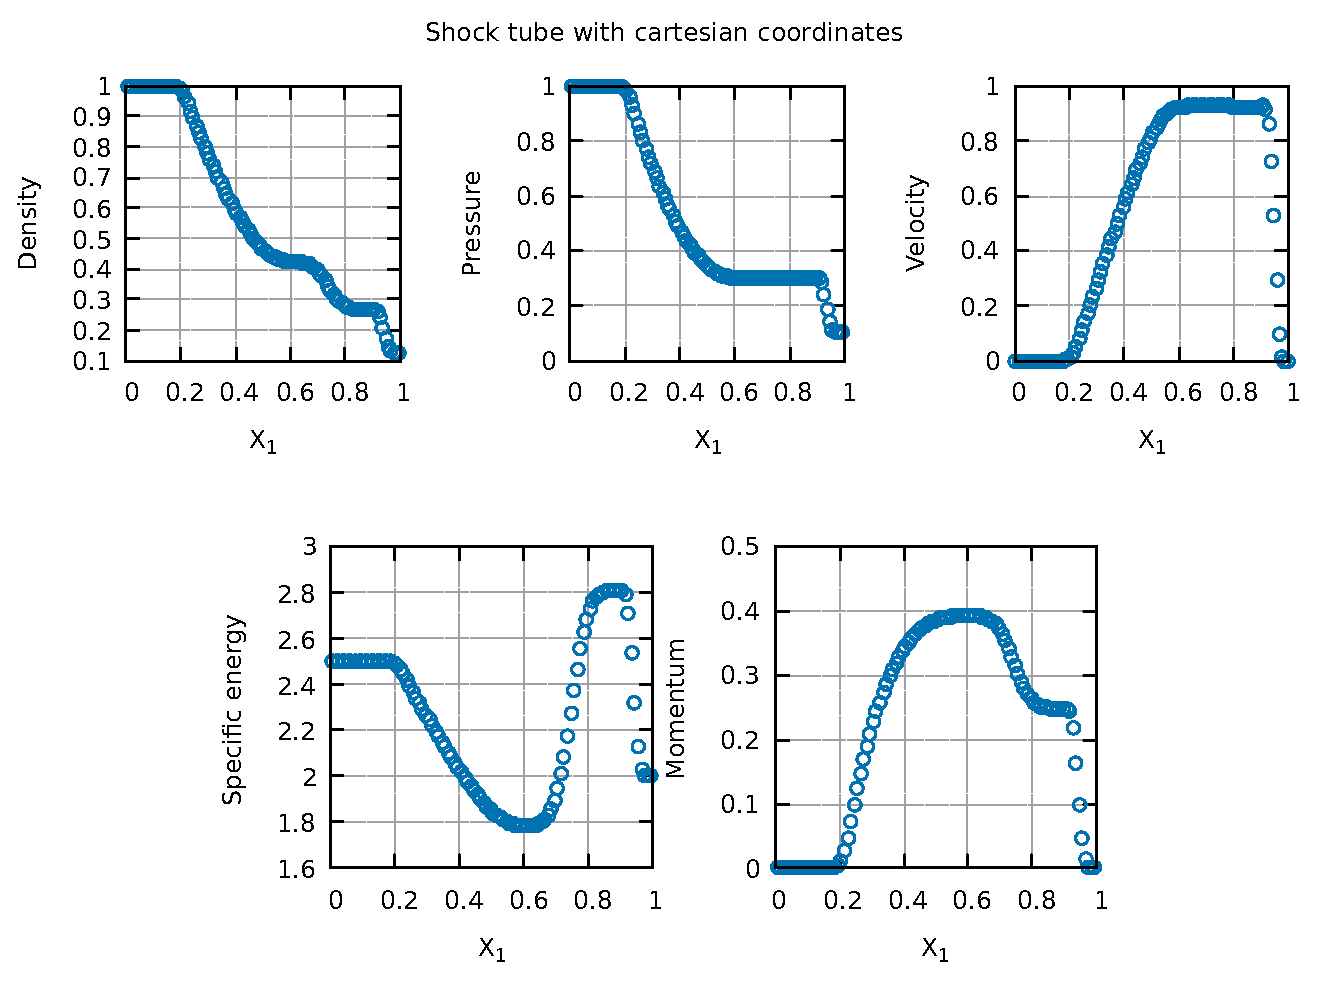
\includegraphics[width=0.8 \linewidth]{cartshock100.pdf}
	\caption{Sod shock tube test for a 100 points grid. From left to right and from top to bottom: $\rho$, $p$, $v$, $\frac{\epsilon}{\rho}$, and $m$ after a $t_{max}=0.245$.}
	\label{fig:cartshock100}
\end{figure}
\begin{figure}[H]
	\centering
	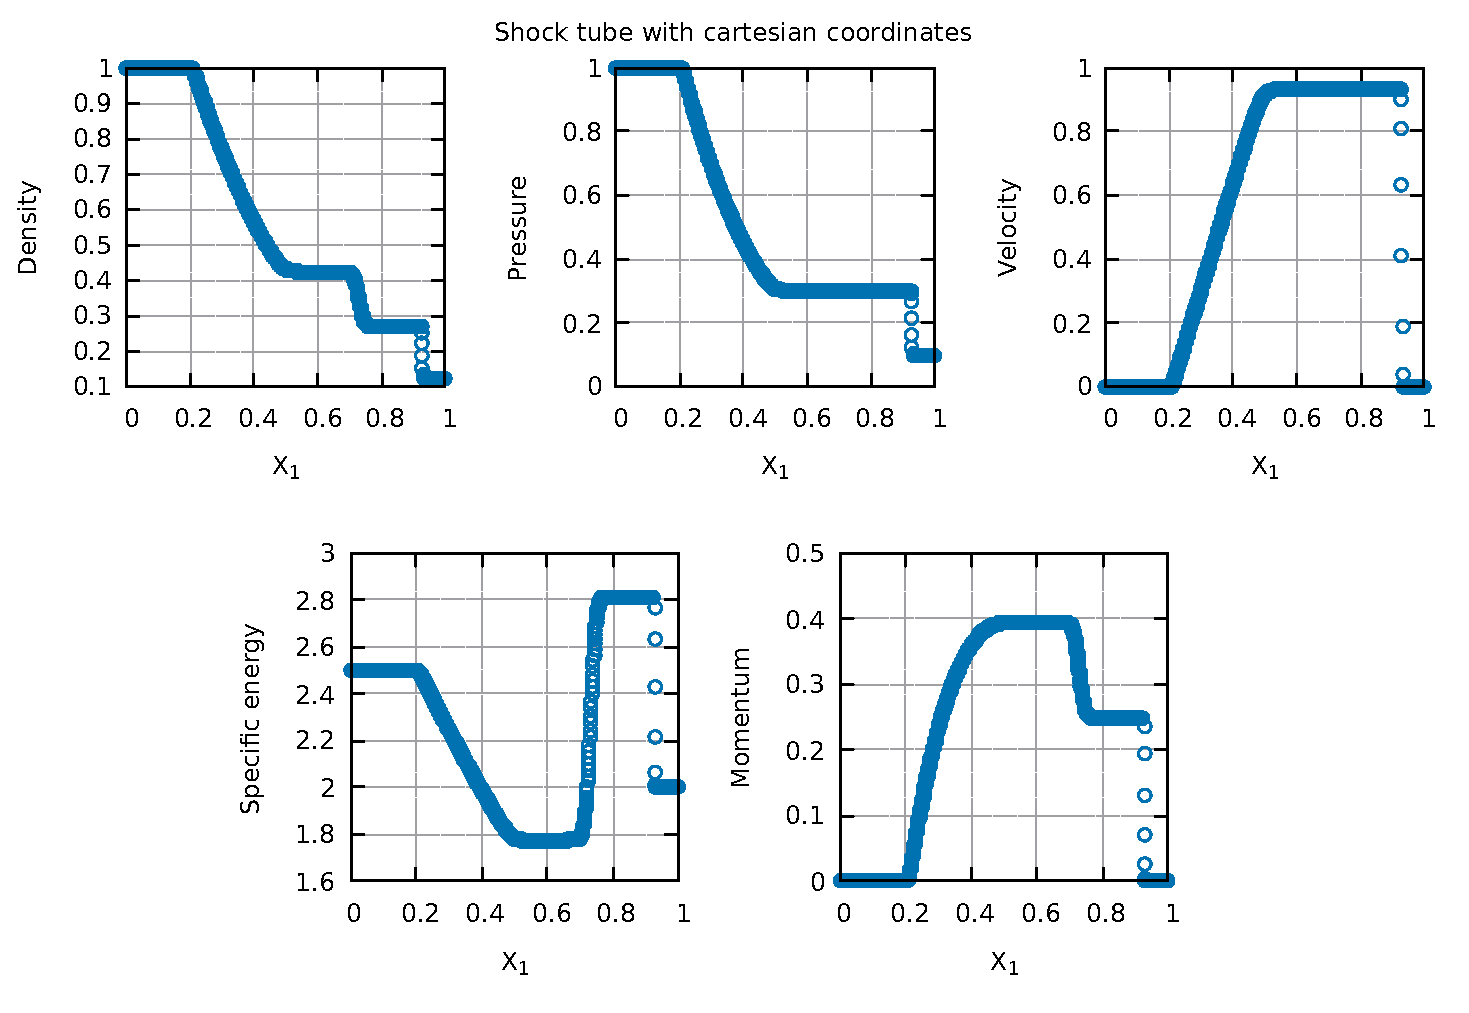
\includegraphics[width=0.8 \linewidth]{cartshock.pdf}
	\caption{Sod shock tube test for a 1000 points grid. From left to right and from top to bottom: $\rho$, $p$, $v$, $\frac{\epsilon}{\rho}$, and $m$ after a $t_{max}=0.245$.}
	\label{fig:cartshock1000}
\end{figure}
\begin{figure}[H]
	\centering
	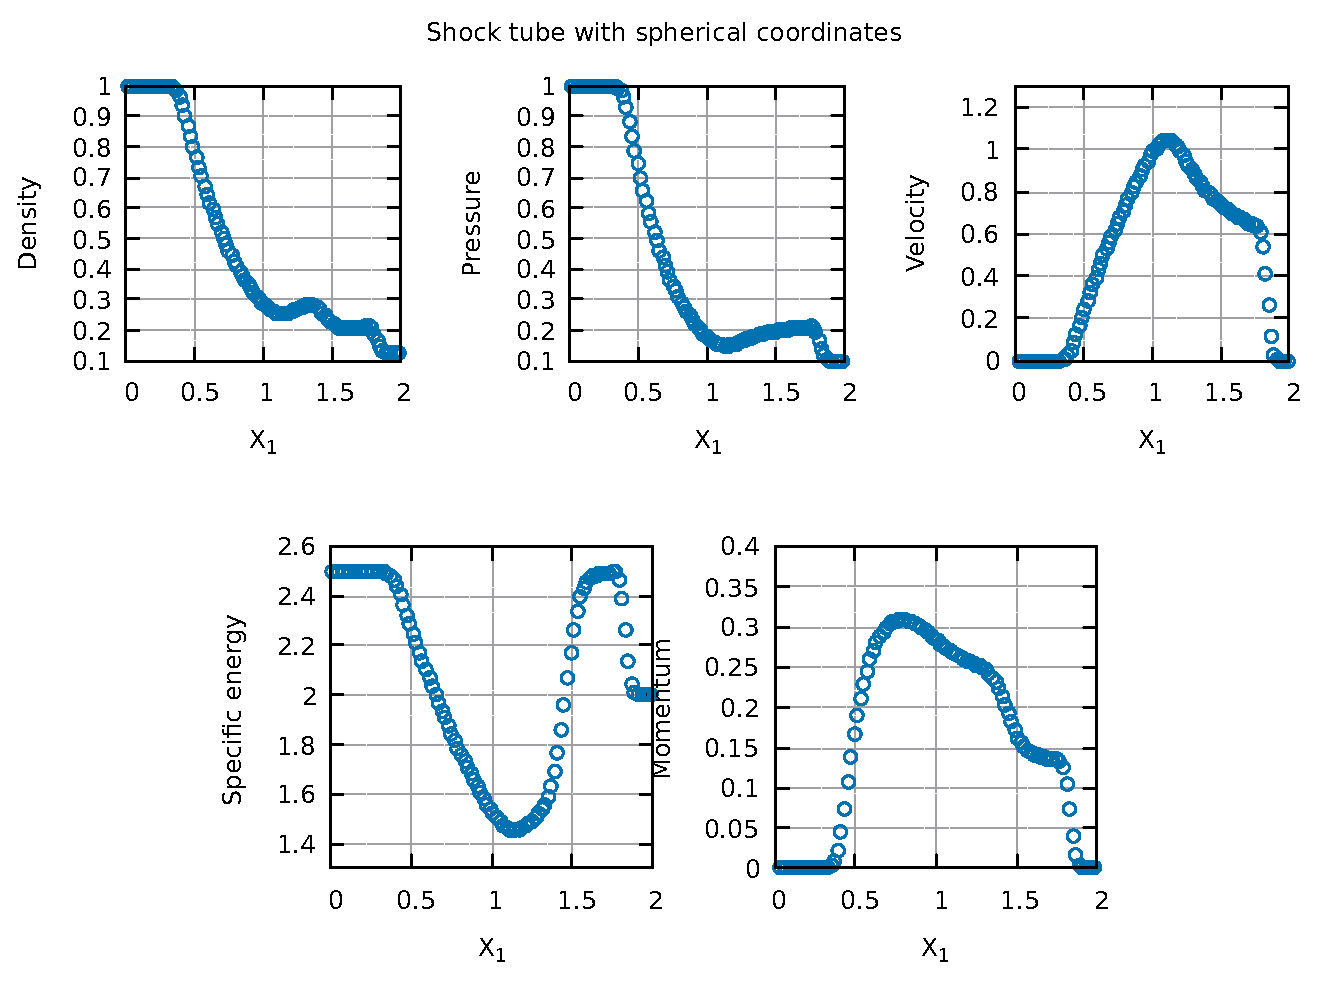
\includegraphics[width=0.8 \linewidth]{spheshock100.pdf}
	\caption{Spherical shock tube test for a 100 points grid. From left to right and from top to bottom: $\rho$, $p$, $v$, $\frac{\epsilon}{\rho}$, and $m$ after a $t_{max}=0.5$.}
	\label{fig:spheshock100}
\end{figure}
\begin{figure}[H]
	\centering
	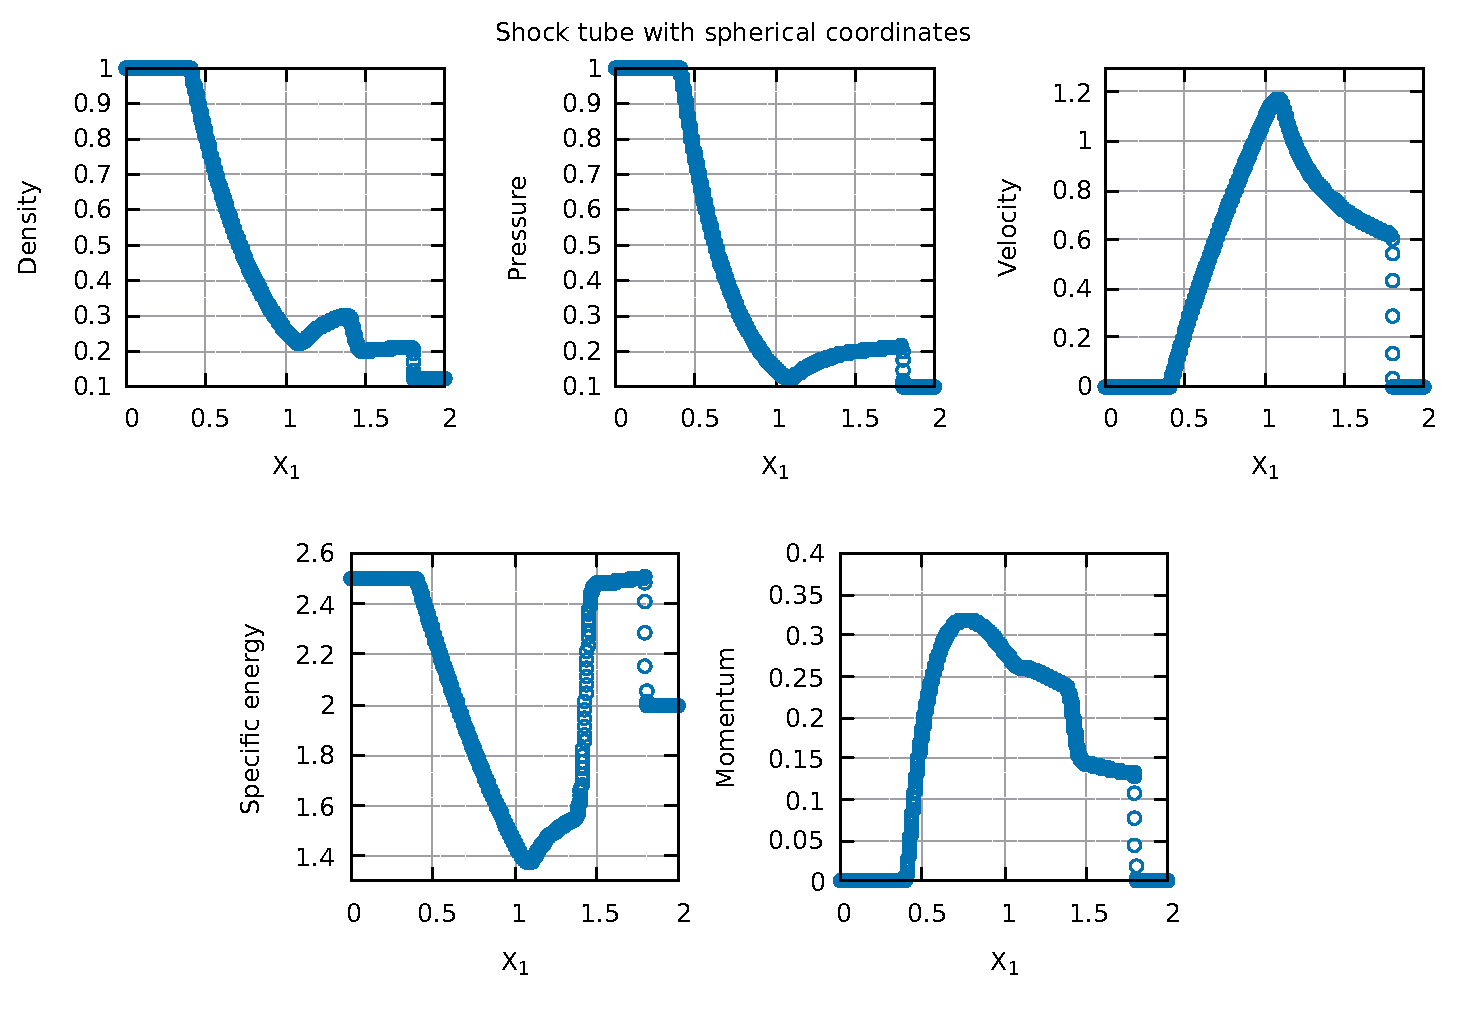
\includegraphics[width=0.8 \linewidth]{spheshock.pdf}
	\caption{Spherical shock tube test for a 1000 points grid. From left to right and from top to bottom: $\rho$, $p$, $v$, $\frac{\epsilon}{\rho}$, and $m$ after a $t_{max}=0.5$.}

	\label{fig:spheshock1000}
\end{figure}
\begin{figure}[H]
	\centering
	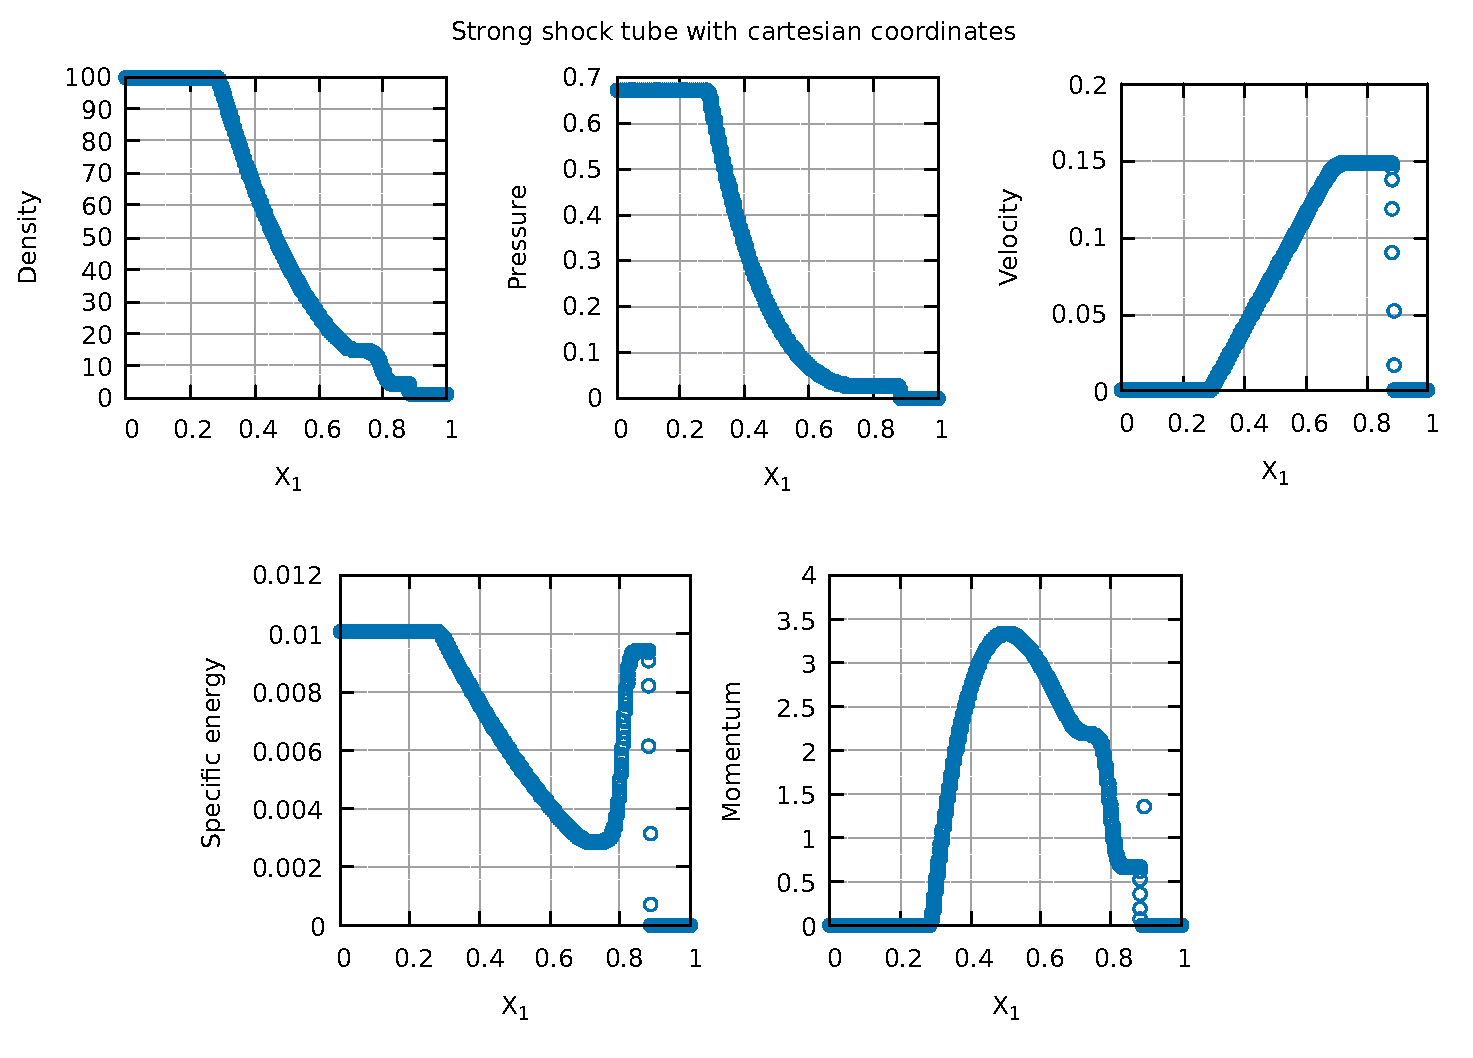
\includegraphics[width=0.8 \linewidth]{strongshocktube.pdf}
	\caption{Strong shock tube test in cartesian coordinates for a 1000 points grid. From left to right and from top to bottom: $\rho$, $p$, $v$, $\frac{\epsilon}{\rho}$, and $m$ after a $t_{max}=2$.}

	\label{fig:strongshock}
\end{figure}
\section{SNR evolution simulation}

\subsection{Physical model}
As mentioned in the introduction, we study the evolution of a SNR, which is divided in different phases. We consider an idealized problem, where a large amount of energy is released in a very small region of an uniform ISM, thus giving us a spherical shock wave, with a very strong shock expected, which allows us to assume that the pressure of the ISM is negligible. \\
The first phase is the free expansion, in which the SN ejecta will expand freely, with $v=v_{ej}$, until it sweeps a mass of ISM comparable to its mass. This means that it terminates when:
\begin{equation}
	\frac{4\pi }{3}R_{1}^{3}\rho_0=M_{ej} \Longrightarrow R_1=\left(\frac{3M_{ej}}{4\pi \rho_0}\right)^{1/3}\sim 2\left(\frac{M_{ej}}{M_{\odot}}\right)^ {1/3}n_0^{-1/3}\; \text{pc},
\end{equation}
where $\rho_0$ is the density of the unperturbed ISM.
Here, we have that the radius is proportional to the time, so the expansion ends at:
\begin{equation}
	t_1=\frac{R_1}{v_{ej}}\sim 200 \left(\frac{M_{ej}}{M_{\odot}}\right)^{1/3}n_0^ {-1/3} \; \text{yr}.
\end{equation}
The second phase is the adiabatic Sedov phase, which is where many observed SNRs are currently at. The ejecta slows down as well as the forward shock, which leaves behind a low-density hot bubble.
Our SNR is basically a bubble with a thin shell in which is where most of the ISM originally contained within the shock radius $R_s$ is. Keeping the assumption of a strong shock and assuming that all of the energy of the SN $E_{SN}$ is contained in the bubble, we find the evolution of the radius now follow a power law, namely the Sedov law:
\begin{equation}
	R_S(t)=1.15\left(\frac{E_{SN}}{\rho_0}\right)^{1/5}t^{2/5}.
\end{equation}
This phase ends when radiative losses become relevant, which is when the temperature of the shock decreases to $T_s\sim10^{6}$ K, which typically happens after a few $10^{4}$ yr, but it has a strong dependance on the density of the ISM. Once radiative cooling becomes important the shell radiates its thermal energy, which causes a decrease in the support against gravity from the pressure and causes the collapse of the structure, making it very cold and dense. This is called radiative shock, where we have that the density is proportional to $\mathcal{M}^2$, where $\mathcal{M}$ is the shock Mach number.
The internal energy loss over time is given by:
\begin{equation}\label{dedt}
	\pdv{\epsilon}{t}= -n^2\Lambda(T)=-\left(\frac{\rho}{2.17\times 10^{-24}\;\text{g$\cdot\,$cm}^{-3}}\right)^2\Lambda(T),
\end{equation}
where $n$ is the number density of the gas particles, and $\Lambda(T)$ is the cooling function. \\
After, the shell continues to expand pushed by the hot, overpressurized bubble; at first, the radius grows as $R_s\propto t^{2/7}$ by adiabatic expansion, then, when the bubble radiates its energy away, the shell expands by momentum conservation, with $R_s\propto t^{1/4}$.

\subsection{The simulation}
We use the usual hydrocode to integrate Euler equations in spherical coordinates. The grid extends from $0$ up to $70$ pc, with $500$ points uniformly spaced. In order to properly deal with the boundary conditions described in Sec.\ref{descrip}, we assign a negative value to the first grid point, i.e. $r_1=-\Delta r$, $r_2=0$, $r_3=\Delta r$, and so on, which makes the point corresponding to $j=3$ the first active point. 
We assume as ISM the ionized Galactic one, so we use its typical values for the initial density $\rho_0$, and temperature $T_0$. In particular, we have $\rho_0=2.0\times 10^{-24}$ g/cm$^{3}$, and $T_0=10^4$ K. Since we're dealing with ionized gas, we have $\gamma =5/3$, and $c_v=2.0\times 10^{51}$ erg$\cdot\,$cm$^{-1}\cdot\,$K$^{-1}$, where $c_v$ is the specific heat capacity at constant volume. We also set out initial velocity to zero, while we derive $p_0$ and $\epsilon_0$ using the relations $\epsilon_0=c_v\rho_0T_0$ and Eq.\eqref{eqstate}. We take $E_0=10^{51}$ erg/s as a value for the energy injected by the SN in the form of thermal energy. Since we assumed this gets injected into a small volume, we consider it to go into the first two active grid points, which numerically means having to change the energy of points 2 and 3 to:
\begin{equation}
	\epsilon_{2+1/2}=\epsilon_{3+1/2}=\frac{E_0}{\frac{4}{3}\pi r_4^3},
\end{equation}
with $T$ and $p$ being updated accordingly.\\
We need a small timestep at the beginning, so we set in Eq.\eqref{timeeq} $C=0.01$ and then we increase it by $10\%$ every cycle up until we get $C=0.5$, then we keep it constant. The artificial viscosity coefficient is still $Q=3$, while we put as total integration time $t_{max}=5\times 10^5$ yr. 
We also modify the code in order to add the possibility of considering the presence of radiative cooling. For the cooling function, we take as reference the one used in \cite{sharma}, which is given by:
\begin{equation}\label{coolfu}
	\Lambda(T)=
	\begin{cases}
		10^{-22}(8.6\times 10^{-3}\,T_{keV}^{-1.7}+0.058\,T_{keV}^{0.5}+0.063)\;\text{erg$\cdot\,$cm$^3\cdot\,$s$^{-1}$} \; &\text{if} \; \;T>0.02\,\text{keV}\\
		6.72\times 10^{-22}(T_{keV}/0.02)^{0.6}\;\text{erg$\cdot\,$cm$^3\cdot\,$s$^{-1}$} \; &\text{if} \; \;T\le0.02\,\text{keV, }T\ge0.0017235\,\text{keV}\\
		1.54\times 10^{-22}(T_{keV}/0.0017235)^{6}\;\text{erg$\cdot\,$cm$^3\cdot\,$s$^{-1}$} \; &\text{if} \; \;T<0.0017235\,\text{keV},
	\end{cases}
\end{equation}
which we plot in Fig.\ref{fig:coolf}.

\begin{figure}[H]
	\centering
	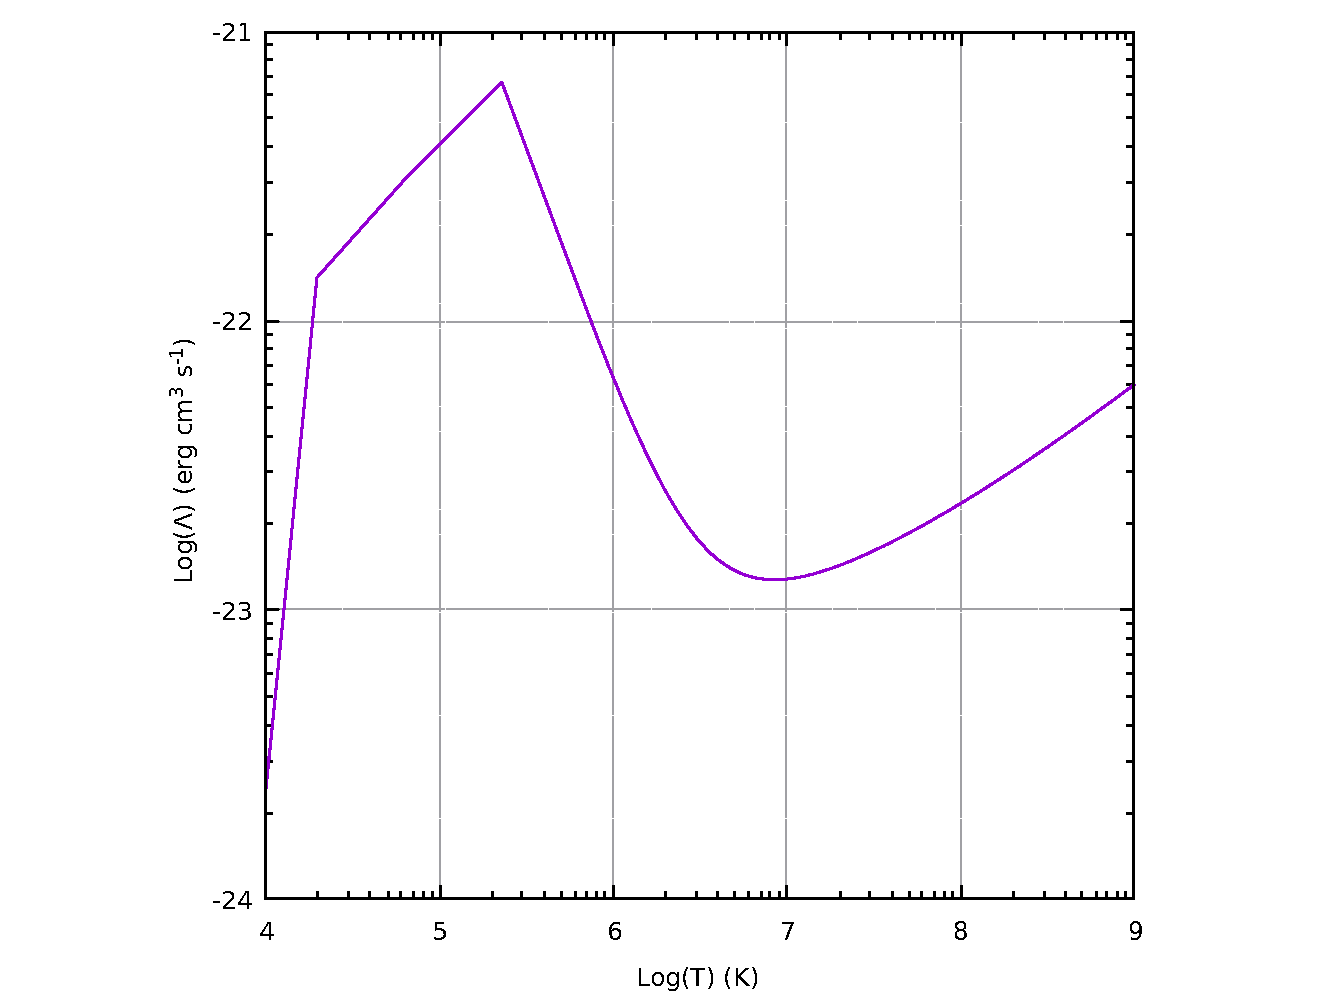
\includegraphics[width=0.7 \linewidth]{coolfunction.pdf}
	\caption{The cooling function defined in Eq.\eqref{coolfu}, plotted for $T<10^9$ K.}
	\label{fig:coolf}
\end{figure}
To implement radiative cooling we transfor Eq.\eqref{dedt} into the following FDE:
\begin{equation}
	\epsilon^{n+1}_{j+1/2}=\epsilon^{n}_{j+1/2}-\Delta t^n\left(\frac{\rho_{j+1/2}}{2.17\times 10^{-24}\text{g}\cdot\text{cm}^{-3}}\right)^2\Lambda(T_{j+1/2}).
\end{equation}
We calculate the following quantities every $10^3$ yr:
\begin{itemize}
	\item the shock radius $R_s$, which we evaluate as the position of the maximum in the density profile;
	\item the thermal $E_{th}$, kinetic $E_{kin}$ and total $E_{tot}$ energy within $r_j$ which are injected in the ISM, which we find using:
			\begin{equation}
				\begin{cases}
					E_{th,1}=E_{th,2}=E_{kin,1}=E_{kin,2}=0\\
					E_{th,j+1}=E_{th,j}+\epsilon_{j+1/2}\frac{4\pi}{3}(r_{j+1}^3-r^3_j)\\
					E_{kin,j+1}=E_{kin}+\frac{1}{2}\rho_{j+1/2}\left(\frac{v_{j+1}+v_j}{2}\right)^2\frac{4\pi}{3}(r_{j+1}^3-r^3_j)\\
					E_{tot,j}=E_{th,j}+E_{kin,j}
				\end{cases}
			\end{equation} 
	\item the X-ray luminosity $L_X$, which we find starting from Eq.\eqref{dedt} and integrating over the volume, however, since below $T=10^6$ K the contribution is negligible, we write the equation for luminosity as:
	\begin{equation}
		\begin{cases}
			L_{X,1}=L_{X,2}=0\\
			L_{X,j+1}=L_{X,j}+\left(\frac{\rho_{j+1/2}}{2.17\times 10^{-24}\text{g}\cdot\text{cm}^{-3}}\right)^2\Lambda(T_{j+1/2})\frac{4\pi}{3}(r_{j+1}^3-r^3_j)\quad &\text{if} \; \;T_{j+1/2}\ge10^6\,\text{K}\\
			L_{X,j+1}=L_{X,j} &\text{otherwise}.
		\end{cases}
	\end{equation} 
\end{itemize}
We will discuss the results in the next section.
\subsection{Results and discussion}
We first show $\rho,\,p,\,v,$ and $T$ as a function of $r$ in the adiabatic case (i.e. the one without radiative cooling). In Fig.\ref{fig:radialpr} we show the plots for $t=10^4,\,2\times10^4,\,4\times10^4,\,6\times10^4,\,8\times 10^4,$ and $10^5$ yr, while in Fig.\ref{fig:radialprhight} we show them for 
$t=2\times10^5,\,3\times10^5,\,4\times10^5,$ and $5\times10^5$ yr. We can clearly see the discrepancies between behind, during, and in front of the shock: behind we have a hot bubble with a low density and nearly constant pressure (which decreases with time), with the shock being characterized with a peak in the density at $\sim 7\times 10^{-24}$ g$\cdot$cm$^{-3}$,
with the profiles of $\rho,\,p,$ and $v$ moving outwards with time, flagging the position of the shell. We can see a progressive decrease in the temperature as the remnant expands.\\
We then show the same profiles but in the case with radiative cooling present. In Fig.\ref{fig:radialprcool} we show the plots for $t=10^4,\,2\times10^4,\,4\times10^4,\,6\times10^4,\,8\times 10^4,$ and $10^5$ yr, while in Fig.\ref{fig:radialprhightcool} we show them for 
$t=2\times10^5,\,3\times10^5,\,4\times10^5,$ and $5\times10^5$ yr. Here, we can see how the density profiles have higher peaks with higher times, which is what we expected in the presence of cooling. \\
\begin{figure}[H] 
	\centering
	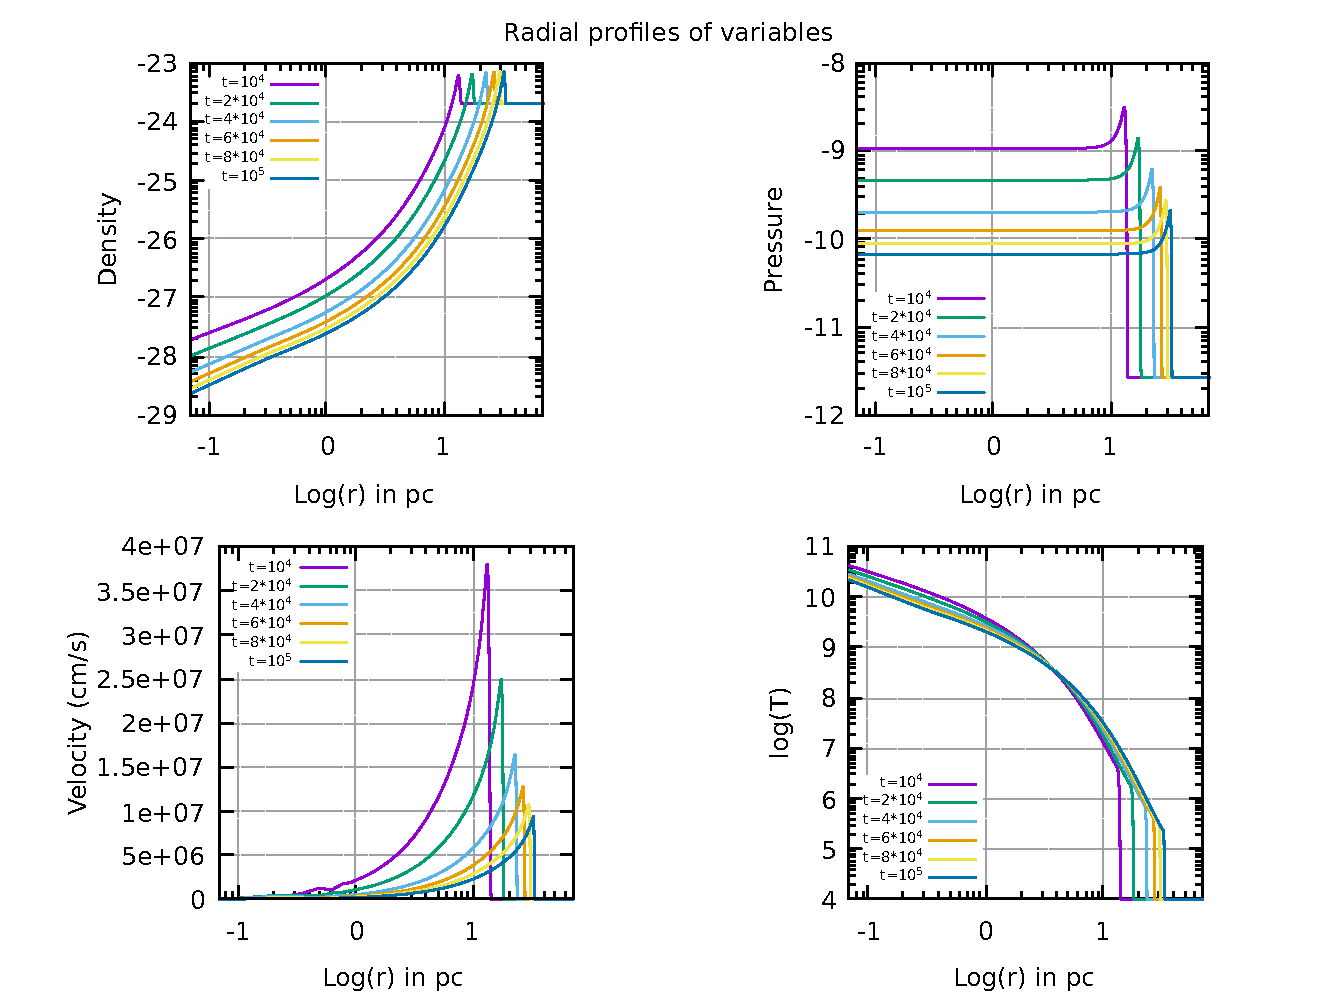
\includegraphics[width=1 \linewidth]{radialprofiles.pdf}
	\caption{From left to right and top to bottom: $\rho,\,p,\,v,$ and $T$ profiles of the ISM computed at times $t=10^4,\,2\times10^4,\,4\times10^4,\,6\times10^4,\,8\times 10^4,$ and $10^5$ yr.}

	\label{fig:radialpr}
\end{figure}
\begin{figure}[H]
	\centering
	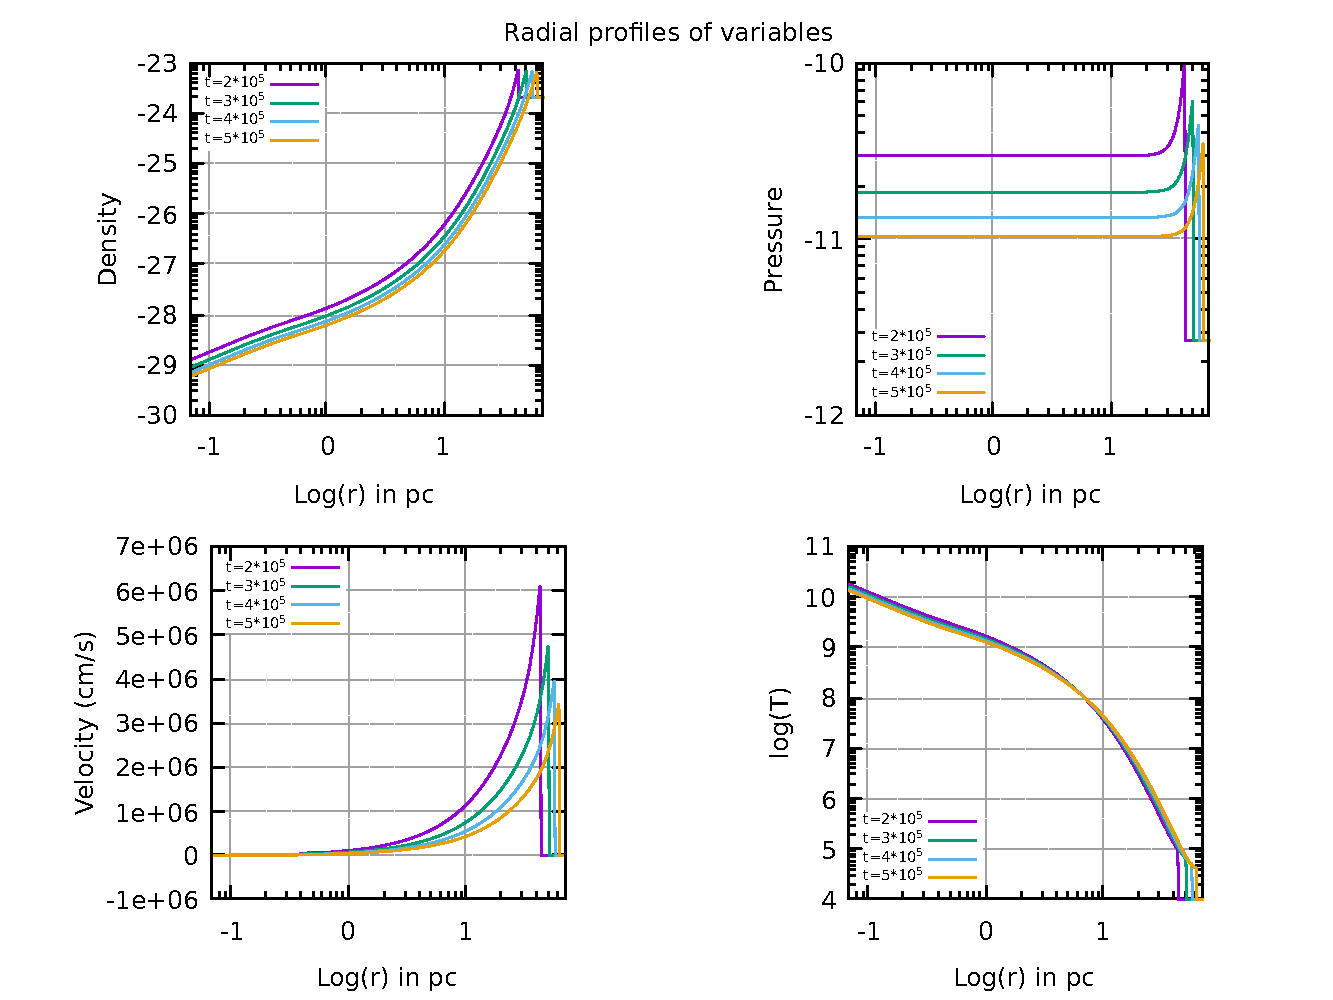
\includegraphics[width=1 \linewidth]{radialprofileshight.pdf}
	\caption{From left to right and top to bottom: $\rho,\,p,\,v,$ and $T$ profiles of the ISM computed at times $t=2\times10^5,\,3\times10^5,\,4\times10^5,$ and $5\times10^5$ yr.}

	\label{fig:radialprhight}
\end{figure}
\begin{figure}[H]
	\centering
	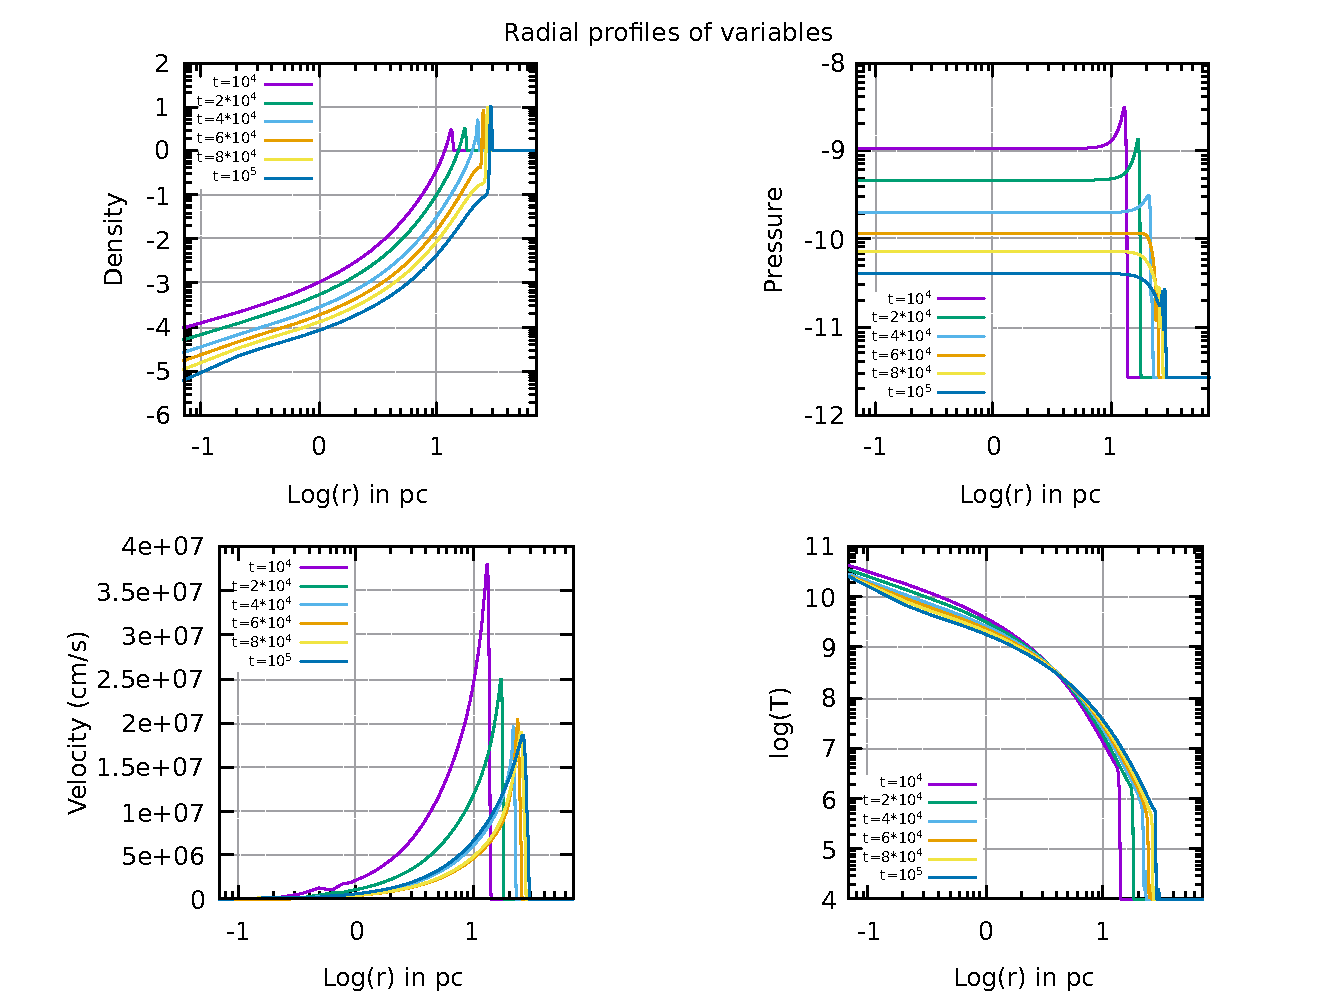
\includegraphics[width=1 \linewidth]{radialprofilescool.pdf}
	\caption{From left to right and top to bottom: $\rho,\,p,\,v,$ and $T$ profiles of the ISM for the radiative cooling model computed at times $t=10^4,\,2\times10^4,\,4\times10^4,\,6\times10^4,\,8\times 10^4,$ and $10^5$ yr.}

	\label{fig:radialprcool}
\end{figure}
\begin{figure}[H]
	\centering
	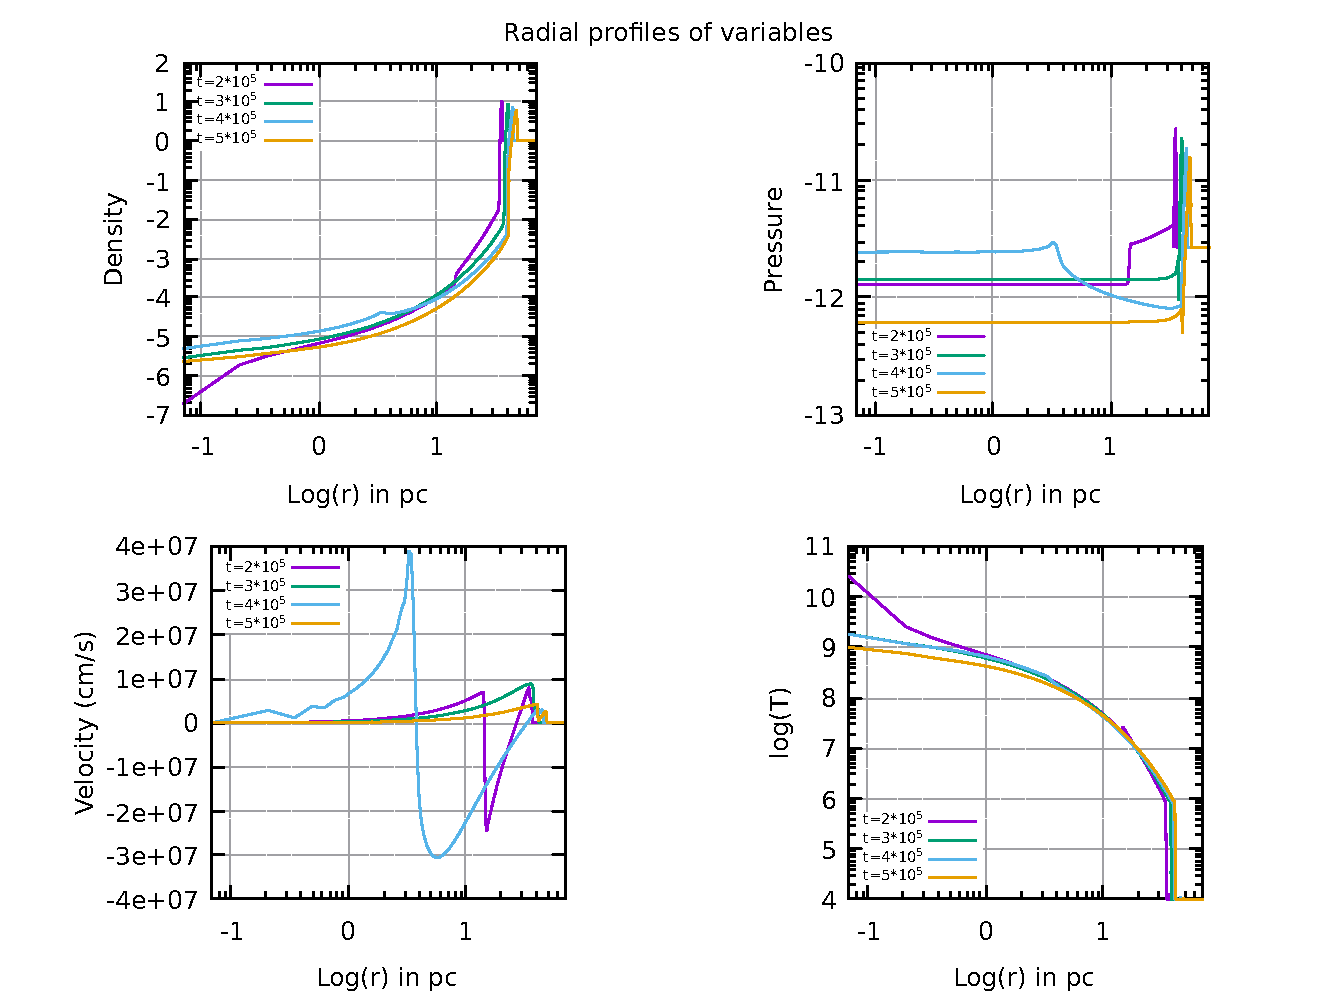
\includegraphics[width=1 \linewidth]{radialprofileshightcool.pdf}
	\caption{From left to right and top to bottom: $\rho,\,p,\,v,$ and $T$ profiles of the ISM for the radiative cooling model computed at times $t=2\times10^5,\,3\times10^5,\,4\times10^5,$ and $5\times10^5$ yr.}


	\label{fig:radialprhightcool}
\end{figure}


In Fig.\ref{fig:sedov} we plot the shock radius as function of time. In the adiabatic case (on the left), we can see how it's pretty much in agreement with the Sedov law; 
we fit the data with a line in the timeranges $t\le3\times 10^{4},$ and $t\ge 2\times 10^5$, obtaining as best fit-values for the time exponent $ 0.3889\pm 0.0009$ and $0.4002\pm 0.0002$ respectively, with both values being really close to the theoretical value $0.4$. On the right we have the case with radiative cooling: here we can see a deviation from the analytical case at around $\sim 3\times 10^4$ yr, which coincide with a drop in the thermal energy, as shown in Fig.\ref{fig:energy} on the right. This means that the ISM retains kinetic energy better than the thermal one. Here, we fit the data with a line in the timeranges $t\le3\times 10^{4},\,3\times10^4\le t\le 10^5,$ and $t\ge 10^5$, obtaining as best fit-values for the time exponent 
$0.3862\pm0.0012$, $0.2863\pm 0.0009$, and $0.3097\pm 0.0002$, which are to be compared to $2/5,\,2/7,$ and $1/4$ respectively.\\
We also checked the conservation of energy as shown in Fig.\ref{fig:energy}, where on the right we have the adiabatic model: we can see that the total energy is not conserved, instead undergoing a slight deacrease, probably due to the fact that we used numerical methods for the simulation. On the right of Fig. \ref{fig:energy} we can instead see the radiative cooling model: as previously mentioned, we can observe a drop in the thermal energy, meaning kinetic energy is better kept in the ISM.\\
The last thing we want to talk about is the X-ray luminosity, plotted in Fig.\ref{fig:luminosity}. The curves show basically the same profile up to the peak at around $t\approx 3\times 10^4$, after which they start to separate due to radiative cooling becoming more effective, causing a faster decrease in temperature. Assuming before and after the peak we can use power laws to describe the luminosity curve (with $L_X\propto t^{\alpha}$), we try to fit the data between $6\times 10^3\le t\le 2.5\times 10^4$ and $3.2\times 10^4\le t\le 10^5$ yr, obtaining $\alpha^{pre}=1.99\pm0.05$, $\alpha^{pre}_{cool}=2.00\pm0.11$, $\alpha^{post}=-3.19\pm0.13$, and $\alpha^{post}_{cool}=-4.55\pm0.19$. We show the fit results in Fig.\ref{fig:luminosityfit}.

\begin{figure}[H]
	\begin{subfigure}{0.5 \linewidth}
		\centering
		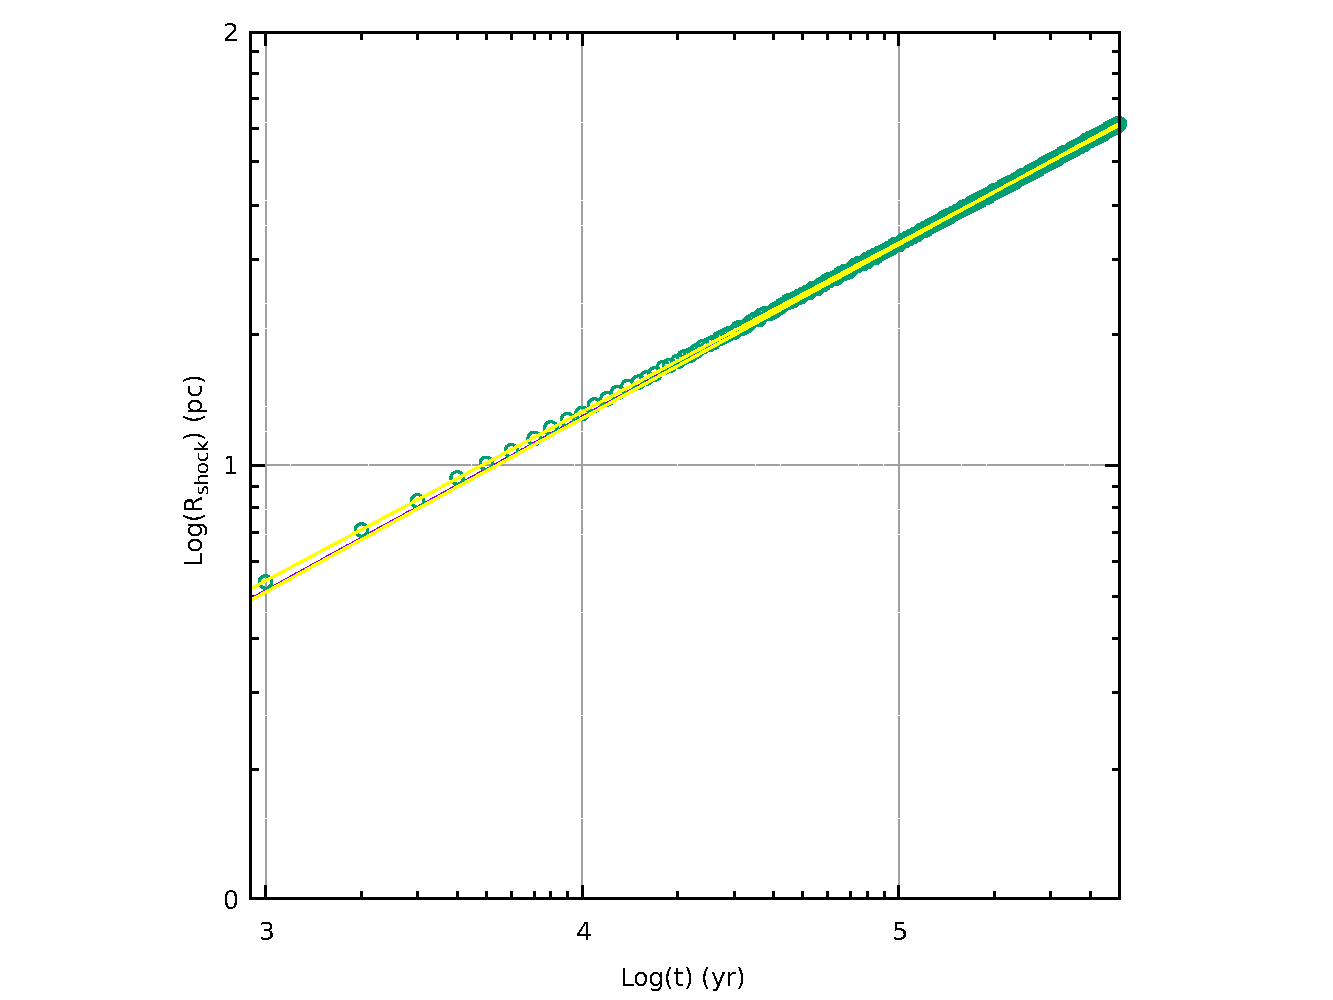
\includegraphics[width=1 \linewidth]{sedov.pdf}
	\end{subfigure}
	\begin{subfigure}{0.5 \linewidth}
		\centering
		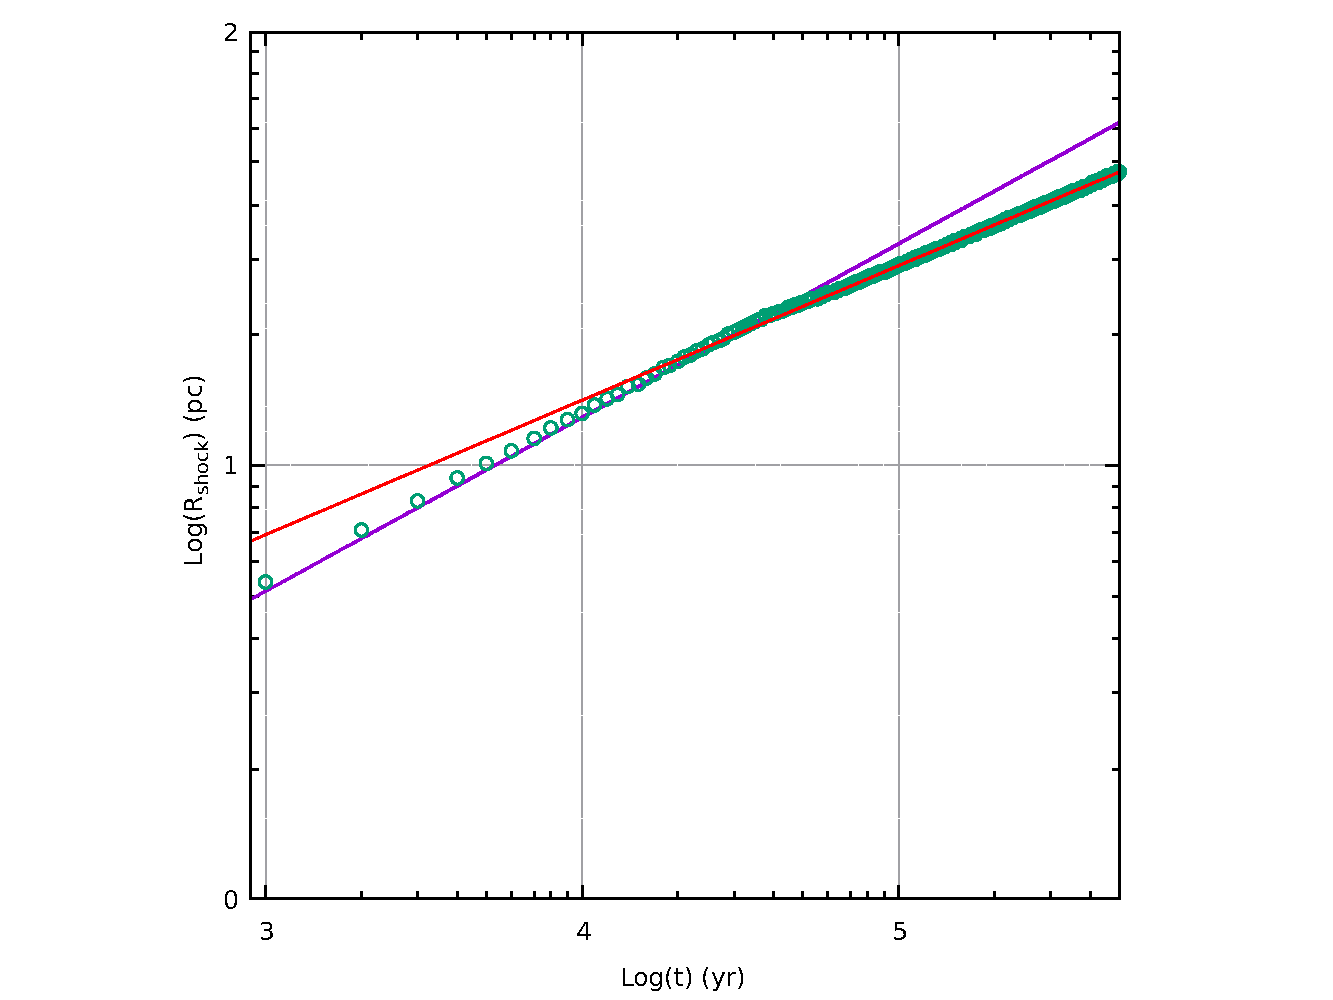
\includegraphics[width=1 \linewidth]{sedovcool.pdf}
	\end{subfigure}
	\caption{The position of $R_s$ as a function of time computed every $10^3$ (green circles). On the left we have the adiabatic model with Sedov law in red and a fitting line going as $\sim t^{2/5}$ in yellow, while on the right we have the model with radiative cooling with the analytical function in purple and a fitting line going as $\sim t^{1/4}$ in red.}

	\label{fig:sedov}
\end{figure}
\begin{figure}[H]
	\begin{subfigure}{0.5 \linewidth}
		\centering
		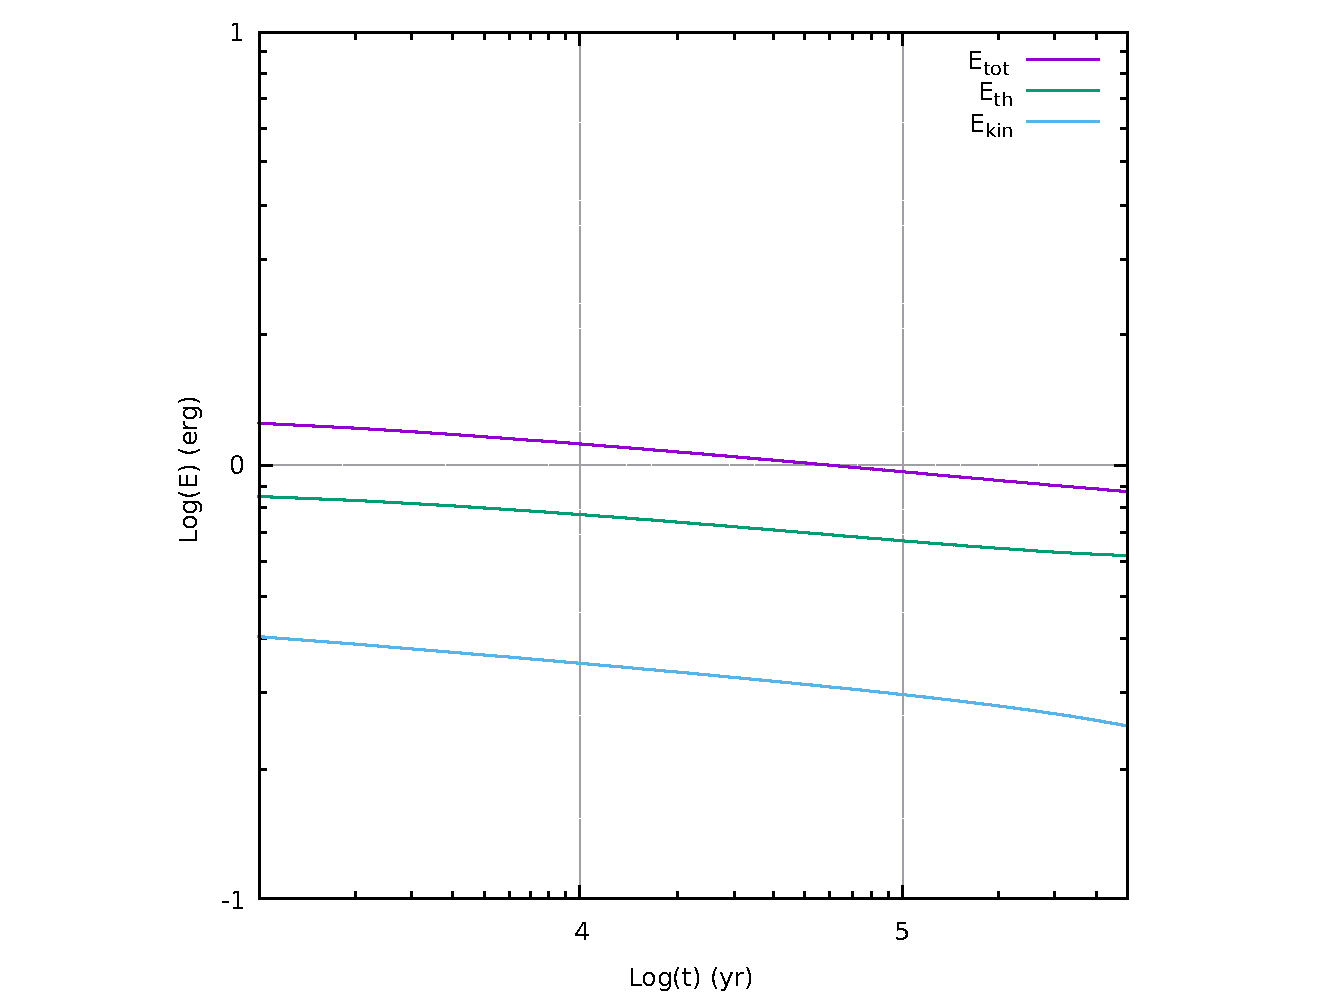
\includegraphics[width=1 \linewidth]{energy.pdf}
	\end{subfigure}
	\begin{subfigure}{0.5 \linewidth}
		\centering
		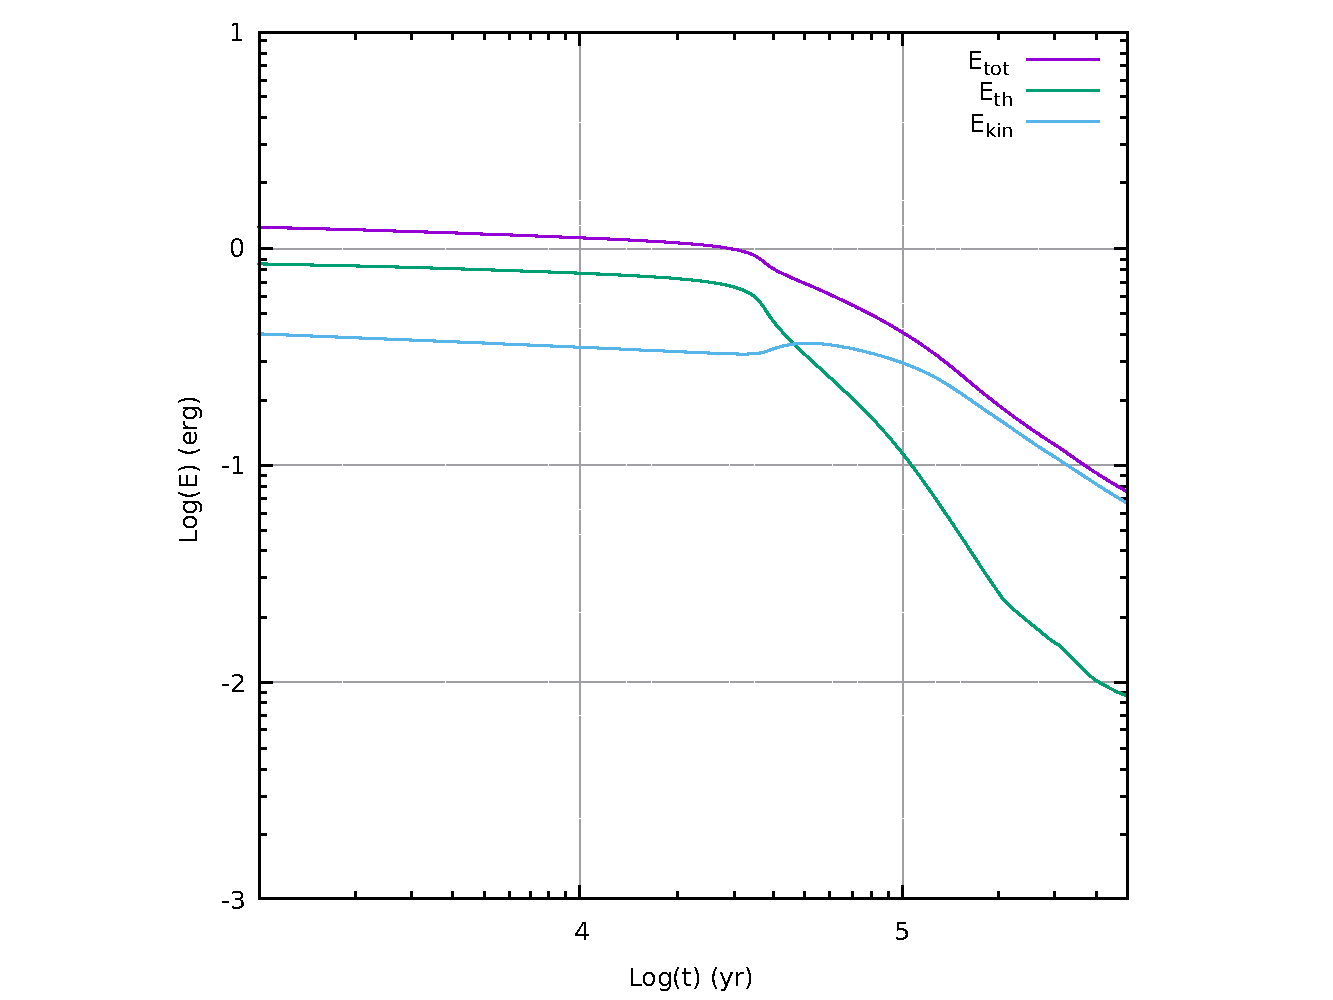
\includegraphics[width=1 \linewidth]{energycool.pdf}
	\end{subfigure}
	\caption{The total SNR energy (purple), the thermal one (green), and the kinetic one (blue) computed every $10^3$ yr for the adiabatic model on the left and for the one with radiative cooling on the right.}

	\label{fig:energy}
\end{figure}
\begin{figure}[H]
	\centering
	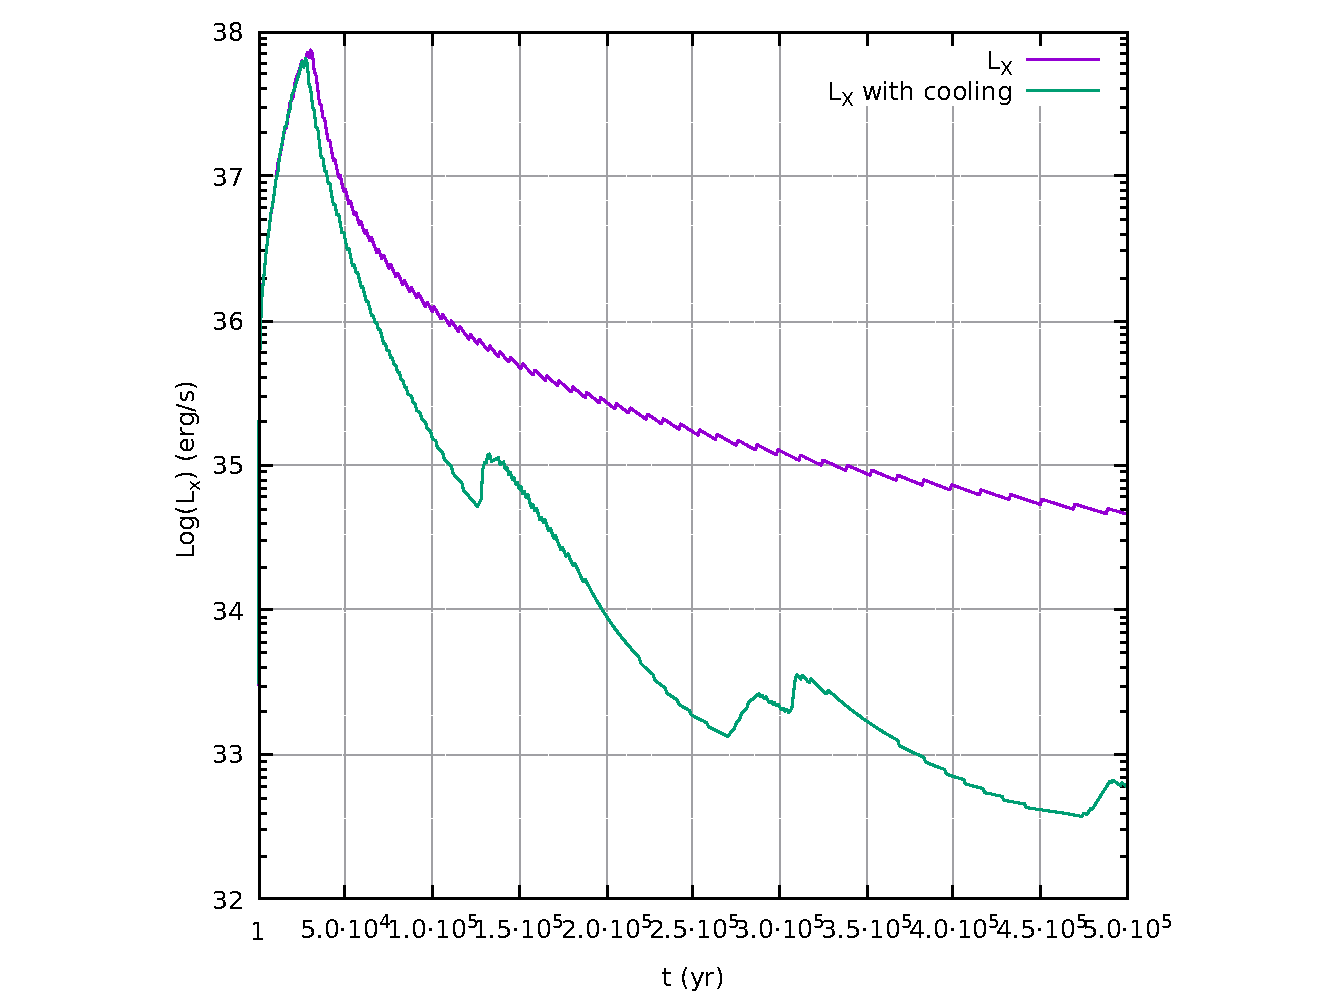
\includegraphics[width=0.6 \linewidth]{luminosity.pdf}
	\caption{The X-ray luminosity as a function of time computed every $10^3$ yr for the adiabatic model (purple) and for the one with radiative cooling (green).}

	\label{fig:luminosity}
\end{figure}

\begin{figure}[H]
	\centering
	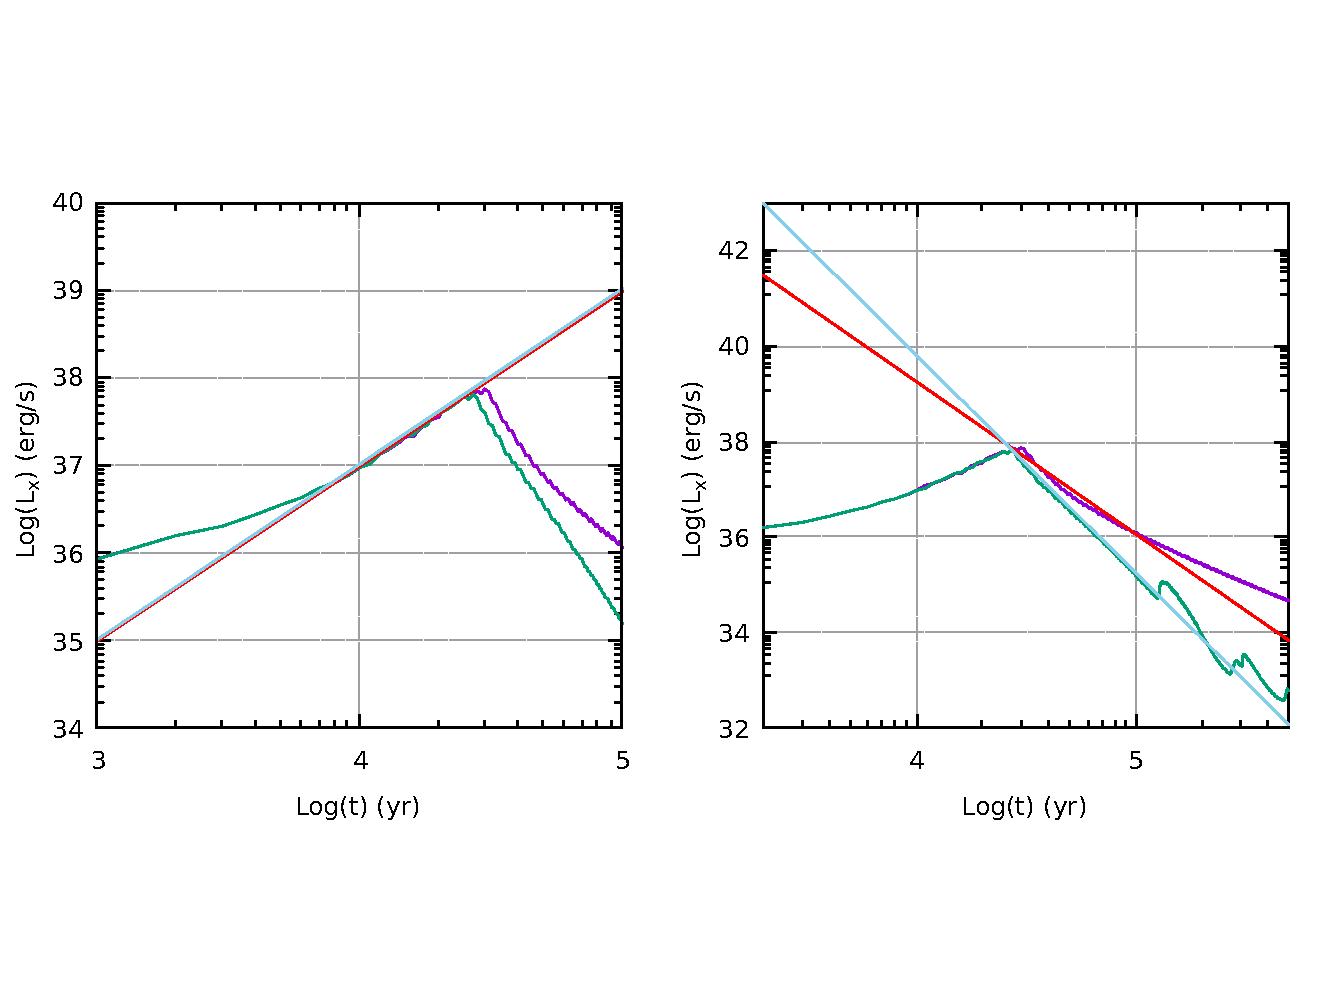
\includegraphics[width=0.8 \linewidth]{luminosityfit.pdf}
	\caption{The X-ray luminosity as a function of time computed every $10^3$ yr for the adiabatic model (purple) and for the one with radiative cooling (green). On the left: best fit lines for before the peak, red for the adiabatic model and lightblue for the one with radiative cooling. On the right:  best fit lines for after the peak, red for the adiabatic model and lightblue for the one with radiative cooling.}

	\label{fig:luminosityfit}
\end{figure}
\section*{Conclusions}
We start with testing a 1D hydrocode, utilizing three different shock tubes. We then try to simulate the evolution of a SNR using numerical simulation for both an adiabatic model and a radiative cooling one, and we show that radiative losses become important after $t\approx 3\times 10^4$ yr after the SN explosion. We also check the evolution of different quantities with their dependance on time, which reproduces the theoretical behaviour, as well as the evolution of the shock radius and how much it's in accordance with the Sedov law except that with cooling it deviates from it at $\sim 3\times 10^4$ yr due to a drop in the thermal energy. We also show the plots with the profiles of the energies, showing that the total energy is unfortunately not conserved, probably due to the numerical origin of the simulation. We lastly show the X-ray luminosity and how it varies when we factor in radiative cooling, obtaining that the latter causes it to decrease faster. 
\begin{thebibliography}{6}
	\bibitem{cimatti}
	A. Cimatti, F. Fraternali, and C. Nipoti. Introduction to Galaxy Formation and Evolution.
From Primordial Gas to Present-Day Galaxies. Cambridge University Press, 2020.
	\bibitem{hawley}
	J. F. Hawley, L. L. Smarr, and J. R. Wilson. “A numerical study of nonspherical
black hole accretion. II - Finite differencing and code calibrations”. In: ApJS
55 (1984), pp. 211–246. doi: https://doi.org/10.1086/190953.
\bibitem{vonneuman}
Von Neumann, J. and Richtmyer, R. D., “A Method for the Numerical Calculation of Hydrodynamic Shocks”, \textit{Journal of Applied Physics}, vol. 21, no. 3, AIP, pp. 232–237, 1950. doi:10.1063/1.1699639.
\bibitem{omang}
M. Omang, J.K. Trulsen, and S. Børve. “SPH in spherical and cylindrical
coordinates”. In: J. Comput. Phys. 213 (2006), pp. 391–412. doi: https :
//doi.org/10.1016/j.jcp.2005.08.023.
\bibitem{sharma}
P. Sharma, I. J. Parrish, and E. Quataert. “Thermal instability with anisotropic
thermal conduction and adiabatic cosmic rays: implications for cold filaments
in galaxy clusters”. In: ApJ 720 (2010), pp. 652–665. doi: https://doi.org/
10.1088/0004-637X/720/1/652.
\bibitem{stone}
J.M. Stone and M. Norman. “Zeus-2D: A radiation magnetohydrodynamics
code for astrophysical flows in two space dimensions. I. The hydrodynamic
algorithms and tests”. In: ApJS 80(2) (1992), pp. 753–790. doi: https://
doi.org/10.1086/191680.
\end{thebibliography}
\end{document}